\section{Experimentación y Resultados}

\subsection{Configuración experimental y selección ex-ante en ENAHO 2024}

\textbf{Entorno reproducible y preprocesamiento interno al pliegue.} Todos los experimentos se ejecutaron en una única corrida sobre un entorno unificado en \textbf{Python 3.12.16 LTS} (\texttt{scikit-learn 1.9.1} \cite{pedregosa2011scikit}, \texttt{lightgbm 4.7.0} \cite{ke2017lightgbm}, \texttt{xgboost 3.4.1} \cite{chen2016xgboost}, \texttt{catboost 1.2.10} \cite{prokhorenkova2018catboost} y \texttt{shap 0.54.1} \cite{lundberg2020local}). Para evitar contención de hilos y fuga de datos, cada pliegue de \texttt{GroupKFold} precalcula estrictamente sobre los índices de entrenamiento cuatro vistas preprocesadas (\texttt{robust\_28}, \texttt{tree\_28}, \texttt{viv\_robust\_11} y \texttt{viv\_tree\_11}), ejecutando la imputación espacial jerárquica (\texttt{conglomerado} $\rightarrow$ \texttt{ubigeo} $\rightarrow$ mediana global) y el escalamiento numérico dentro del pliegue. Una verificación previa en \texttt{GroupKFold(5)} sobre ENAHO 2024 confirmó que \texttt{RobustScaler} supera o iguala a \texttt{StandardScaler} y \texttt{MinMaxScaler} en modelos sensibles a escala (\texttt{PR-AUC OOF} de $0.5790$ frente a $0.5789$ y $0.5764$ en logística ElasticNet; $0.5567$ frente a $0.5432$ y $0.5313$ en perceptrón multicapa), validando su adopción frente a la asimetría en tamaño de hogar y dependencia.

\begin{figure*}[!t]
\centering
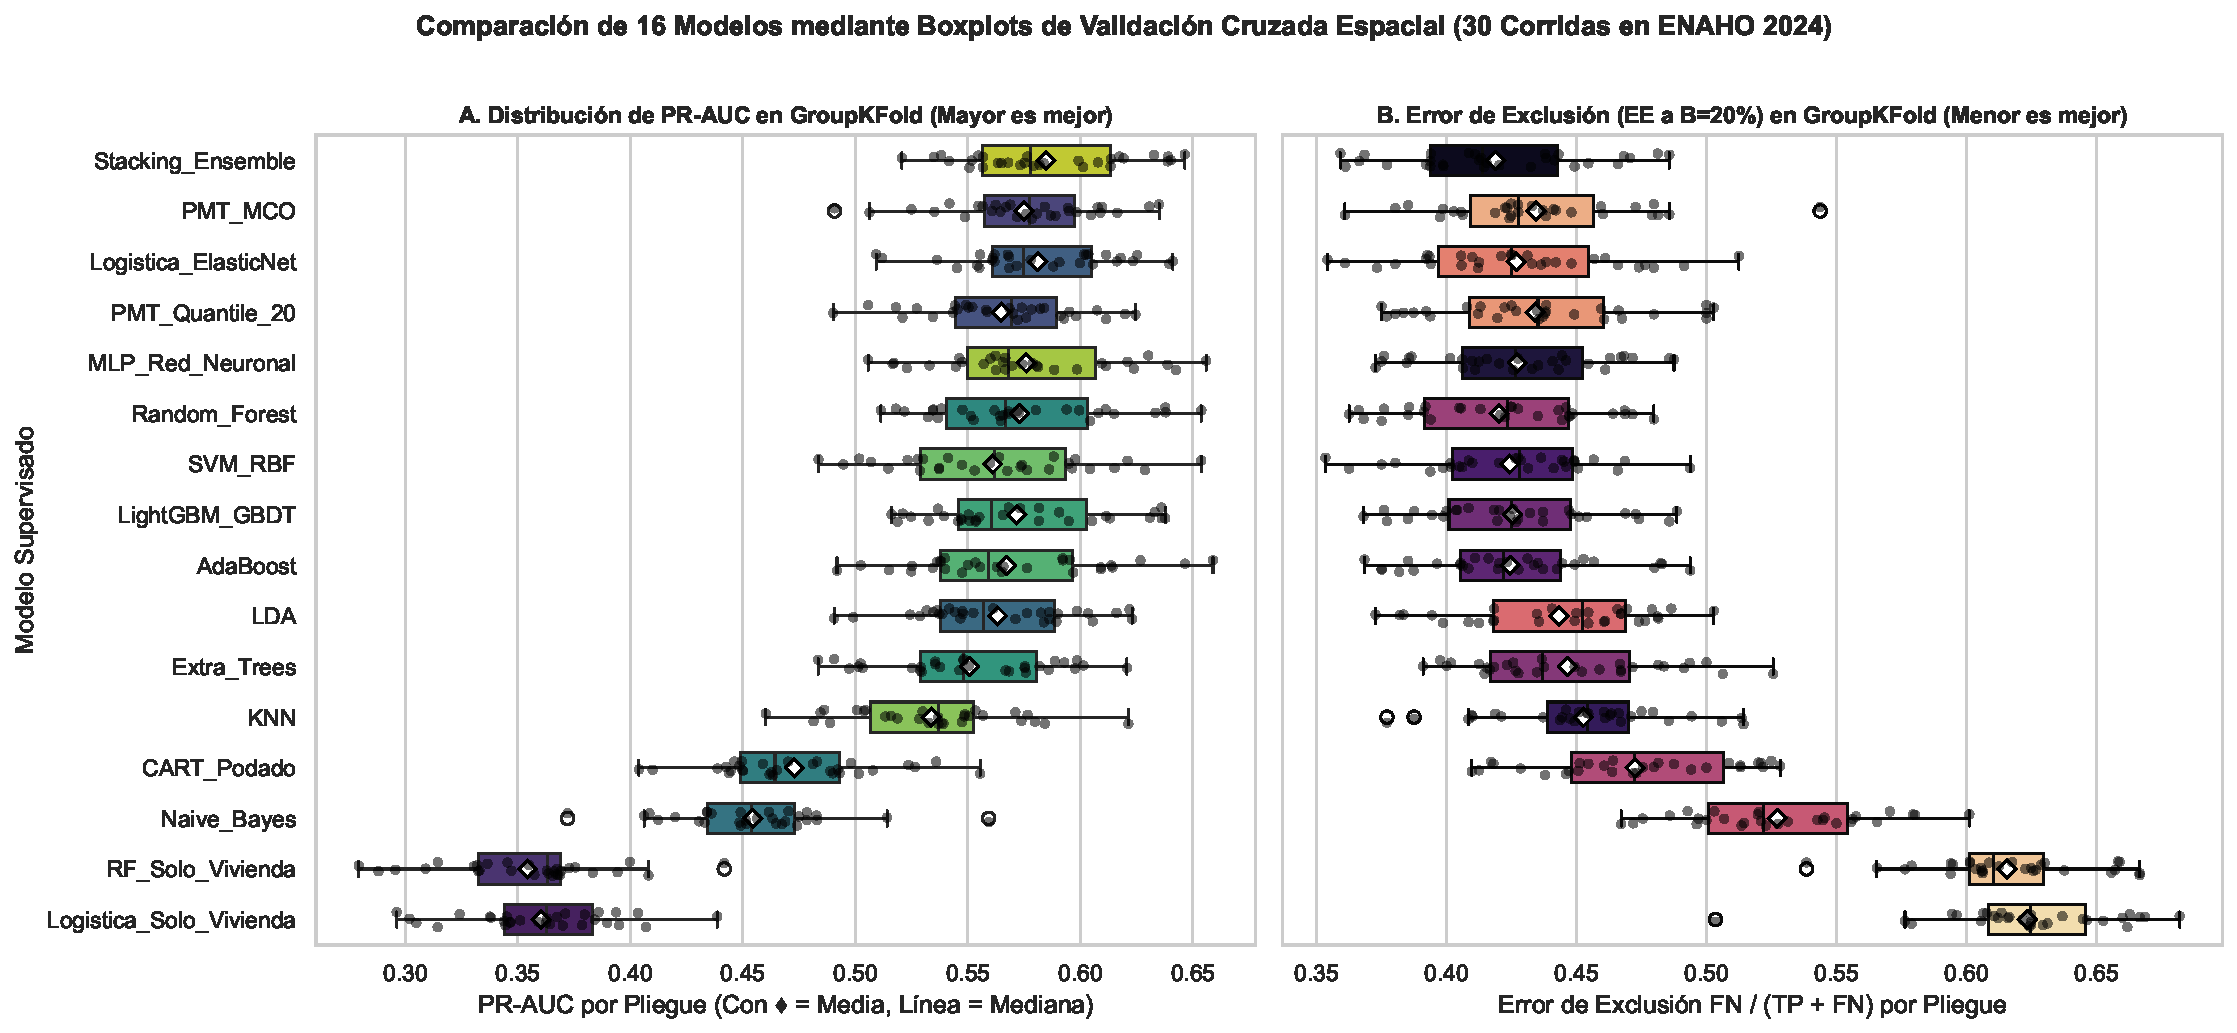
\includegraphics[width=0.90\textwidth,height=0.225\textheight,keepaspectratio]{figures/cv2024_boxplot_models.pdf}
\caption{Distribución de desempeño de los 19 modelos sobre las 30 corridas de Validación Cruzada Espacial Repetida ($6\times 5$ pliegues agrupados por conglomerado) en ENAHO 2024 ($N=4{,}090$). Izquierda (Panel A): PR-AUC por pliegue. Derecha (Panel B): Error de Exclusión a cobertura presupuestal fija $B=20\%$.}
\label{fig:cv2024_boxplots}
\end{figure*}

\textbf{Benchmark de 19 modelos y selección ex-ante en 2024.} Sobre la ENAHO 2024 ($N=4{,}090$ hogares, 704 conglomerados, prevalencia de pobreza $18.92\%$) se evaluaron primero las 99 configuraciones candidatas en \texttt{GroupKFold(5)} para seleccionar la configuración óptima de cada uno de los 19 algoritmos según PR-AUC fuera de pliegue. En dicha partición única de 5 pliegues, \texttt{Logistica\_ElasticNet} obtuvo la mayor \texttt{PR-AUC OOF} ($0.5796$), seguida por \texttt{XGBoost\_GBDT} ($0.5737$), \texttt{Stacking\_Ensemble} ($0.5722$), \texttt{PMT\_MCO} ($\alpha_{\text{ridge}}=10$, $0.5720$), \texttt{CatBoost\_GBDT} ($0.5717$) y \texttt{LightGBM\_GBDT} ($0.5609$). A continuación, aplicando la \textbf{regla formal de selección ex-ante} sobre las \textbf{30 corridas de Validación Cruzada Espacial Repetida} ($6\text{ repeticiones}\times 5\text{ pliegues} = 570\text{ evaluaciones}$ en 2024, Figura~\ref{fig:cv2024_boxplots}), \textbf{\texttt{Stacking\_Ensemble}} resultó elegido como modelo ganador al registrar la mayor mediana de PR-AUC ($0.5797$, $\text{IQR}=0.0365$, media $0.5851$, rango medio de Friedman $4.53$ y mediana de $\text{EE}_{B=20\%}=0.4138$). Como muestra la Tabla~\ref{tab:resultados_2024_2025}, existe un empate estadístico técnico en la cúspide entre \texttt{Stacking\_Ensemble}, \texttt{XGBoost\_GBDT} (mediana $0.5788$, mejor media $0.5868$, mejor rango de Friedman $4.23$ y Wilcoxon $p=0.3818$), \texttt{CatBoost\_GBDT} (mediana $0.5751$, menor mediana de $\text{EE}_{B=20\%}=0.4103$, $p=0.5028$), \texttt{Logistica\_ElasticNet} (mediana $0.5744$, $p=0.3285$) y \texttt{LightGBM\_GBDT} (mediana $0.5722$, $p=0.1347$). En contraste, los modelos restringidos a las 11 variables de vivienda (\texttt{RF\_Solo\_Vivienda} $0.3640$ y \texttt{Logistica\_Solo\_Vivienda} $0.3629$) quedan más de $21$ puntos de PR-AUC por debajo ($p = 1.86\times 10^{-9}$).

\begin{table*}[!t]
\centering
\caption{Desempeño comparativo en validación espacial ENAHO 2024 ($N=4{,}090$, 30 corridas y 5-fold OOF) y evaluación ciega fuera de tiempo ENAHO 2025 sin hogares panel ($N=3{,}199$, 601 conglomerados). Se incluyen los 12 mejores modelos en $\mathbb{R}^{28}$ y las dos líneas base solo vivienda ($H_1$).}
\label{tab:resultados_2024_2025}
\fontsize{6.4}{7.8}\selectfont
\setlength{\tabcolsep}{2.4pt}
\begin{tabular}{lccccccccccccc}
\toprule
& \multicolumn{5}{c}{\textbf{Validación Espacial ENAHO 2024 (Ex-Ante)}} & \multicolumn{8}{c}{\textbf{Evaluación Ciega Fuera de Tiempo ENAHO 2025 ($N_{\text{test}}=3{,}199$)}} \\
\cmidrule(lr){2-6}\cmidrule(lr){7-14}
\textbf{Modelo} & \textbf{PR Med.} & \textbf{Rank} & \textbf{Wilcox.} & \textbf{PR OOF} & $\boldsymbol{\tau_{2024}}$ & \textbf{PR 2025} & \textbf{PR Pond.} & $\boldsymbol{\Delta_{\text{temp}}}$ & \textbf{ROC 2025} & \textbf{EE B20} & \textbf{EE Pond.} & \textbf{Rec. $\boldsymbol{\tau}$} & \textbf{Prec. $\boldsymbol{\tau}$} \\
\midrule
\textbf{Stacking\_Ensemble (Ganador)} & \textbf{0.5797} & 4.53 & 1.0000 & 0.5722 & 0.2060 & 0.5642 & 0.5536 & 0.0080 & 0.8593 & 0.4057 & \textbf{0.4480} & 0.7110 & 0.4573 \\
\textbf{XGBoost\_GBDT} & 0.5788 & \textbf{4.23} & 0.3818 & 0.5737 & 0.4112 & \textbf{0.5683} & \textbf{0.5639} & 0.0054 & 0.8561 & 0.4057 & 0.4565 & 0.7002 & 0.4561 \\
\textbf{PMT\_MCO (OLS/Ridge)} & 0.5773 & 6.70 & 0.0345 & 0.5720 & 0.2419 & 0.5558 & 0.5432 & 0.0162 & \textbf{0.8597} & 0.4057 & 0.4597 & 0.7074 & \textbf{0.4619} \\
\textbf{CatBoost\_GBDT} & 0.5751 & 5.50 & 0.5028 & 0.5717 & 0.5688 & 0.5604 & 0.5561 & 0.0114 & 0.8554 & 0.4075 & 0.4577 & 0.7127 & 0.4511 \\
\textbf{Logistica\_ElasticNet} & 0.5744 & 5.13 & 0.3285 & \textbf{0.5796} & 0.3738 & 0.5543 & 0.5414 & 0.0253 & 0.8556 & \textbf{0.3932} & 0.4525 & \textbf{0.7289} & 0.4462 \\
\textbf{LightGBM\_GBDT} & 0.5722 & 5.87 & 0.1347 & 0.5609 & 0.3950 & 0.5587 & 0.5558 & 0.0022 & 0.8506 & 0.4093 & 0.4677 & 0.7092 & 0.4530 \\
PMT\_Quantile\_20 & 0.5694 & 9.60 & $<0.001$ & 0.5591 & 0.2402 & 0.5359 & 0.5240 & 0.0233 & 0.8516 & 0.4129 & 0.4566 & 0.6912 & 0.4513 \\
MLP\_Red\_Neuronal & 0.5680 & 6.77 & 0.0137 & 0.5609 & 0.2732 & 0.5314 & 0.5262 & 0.0295 & 0.8461 & 0.4057 & 0.4570 & 0.6463 & 0.4839 \\
\textbf{Random\_Forest} & 0.5659 & 7.97 & $<0.001$ & 0.5569 & 0.5454 & 0.5489 & 0.5397 & 0.0080 & 0.8545 & 0.4075 & 0.4571 & 0.7002 & 0.4457 \\
SVM\_RBF & 0.5615 & 10.33 & $<0.001$ & 0.5476 & 0.2207 & 0.5472 & 0.5433 & \textbf{0.0004} & 0.8475 & 0.4057 & 0.4601 & 0.7020 & 0.4562 \\
HistGBDT\_Sklearn & 0.5604 & 8.60 & 0.0030 & 0.5569 & 0.2549 & 0.5532 & 0.5526 & 0.0037 & 0.8514 & 0.4057 & 0.4696 & 0.7038 & 0.4501 \\
\textbf{CART\_Podado} & 0.4647 & 16.23 & $<0.001$ & 0.4587 & 0.5815 & 0.4305 & 0.4408 & 0.0282 & 0.8035 & 0.4632 & 0.5019 & 0.7074 & 0.3770 \\
\addlinespace[1.5pt]
Logistica\_Solo\_Vivienda ($H_1$) & 0.3629 & 18.37 & $<0.001$ & 0.3580 & 0.5148 & 0.3440 & 0.3499 & 0.0140 & 0.7390 & 0.5817 & 0.6374 & 0.7217 & 0.3041 \\
RF\_Solo\_Vivienda ($H_1$) & 0.3640 & 18.63 & $<0.001$ & 0.3418 & 0.5397 & 0.3367 & 0.3448 & 0.0051 & 0.7345 & 0.5907 & 0.6436 & 0.7181 & 0.2935 \\
\bottomrule
\end{tabular}
\end{table*}

\subsection{Evaluación ciega fuera de tiempo (ENAHO 2025) y curvas de focalización}

Al evaluar sin reajuste los modelos entrenados en 2024 sobre los $N_{\text{test}}=3{,}199$ hogares independientes de la ENAHO 2025 ($557$ hogares pobres, $17.41\%$), los resultados confirman una generalización interanual sólida (Tabla~\ref{tab:resultados_2024_2025}). \texttt{XGBoost\_GBDT} alcanza la mayor PR-AUC en 2025 tanto a nivel muestral ($0.5683$) como ponderada por factor de expansión \texttt{FACTOR07} ($0.5639$), mientras que el ganador ex-ante \textbf{\texttt{Stacking\_Ensemble}} se ubica en segundo lugar general ($0.5642$ muestral y $0.5536$ ponderada) y logra el \textbf{menor error de exclusión poblacional ponderado a $B=20\%$} ($\text{EE}_{\text{Pond}}=0.4480$), además de una excelente calibración probabilística ($\text{Brier}=0.1051$, solo superada por $0.1047$ de \texttt{PMT\_MCO}). \texttt{CatBoost\_GBDT} ($0.5604$), \texttt{LightGBM\_GBDT} ($0.5587$), \texttt{PMT\_MCO} ($0.5558$, mayor $\text{ROC-AUC}=0.8597$) y \texttt{Logistica\_ElasticNet} ($0.5543$, menor error de exclusión muestral $\text{EE}_{B=20\%}=0.3932$ e $\text{IE}_{B=20\%}=0.4719$) conforman un bloque compacto cuya diferencia máxima en PR-AUC es de apenas $1.4$ puntos porcentuales.

\begin{figure*}[!t]
\centering
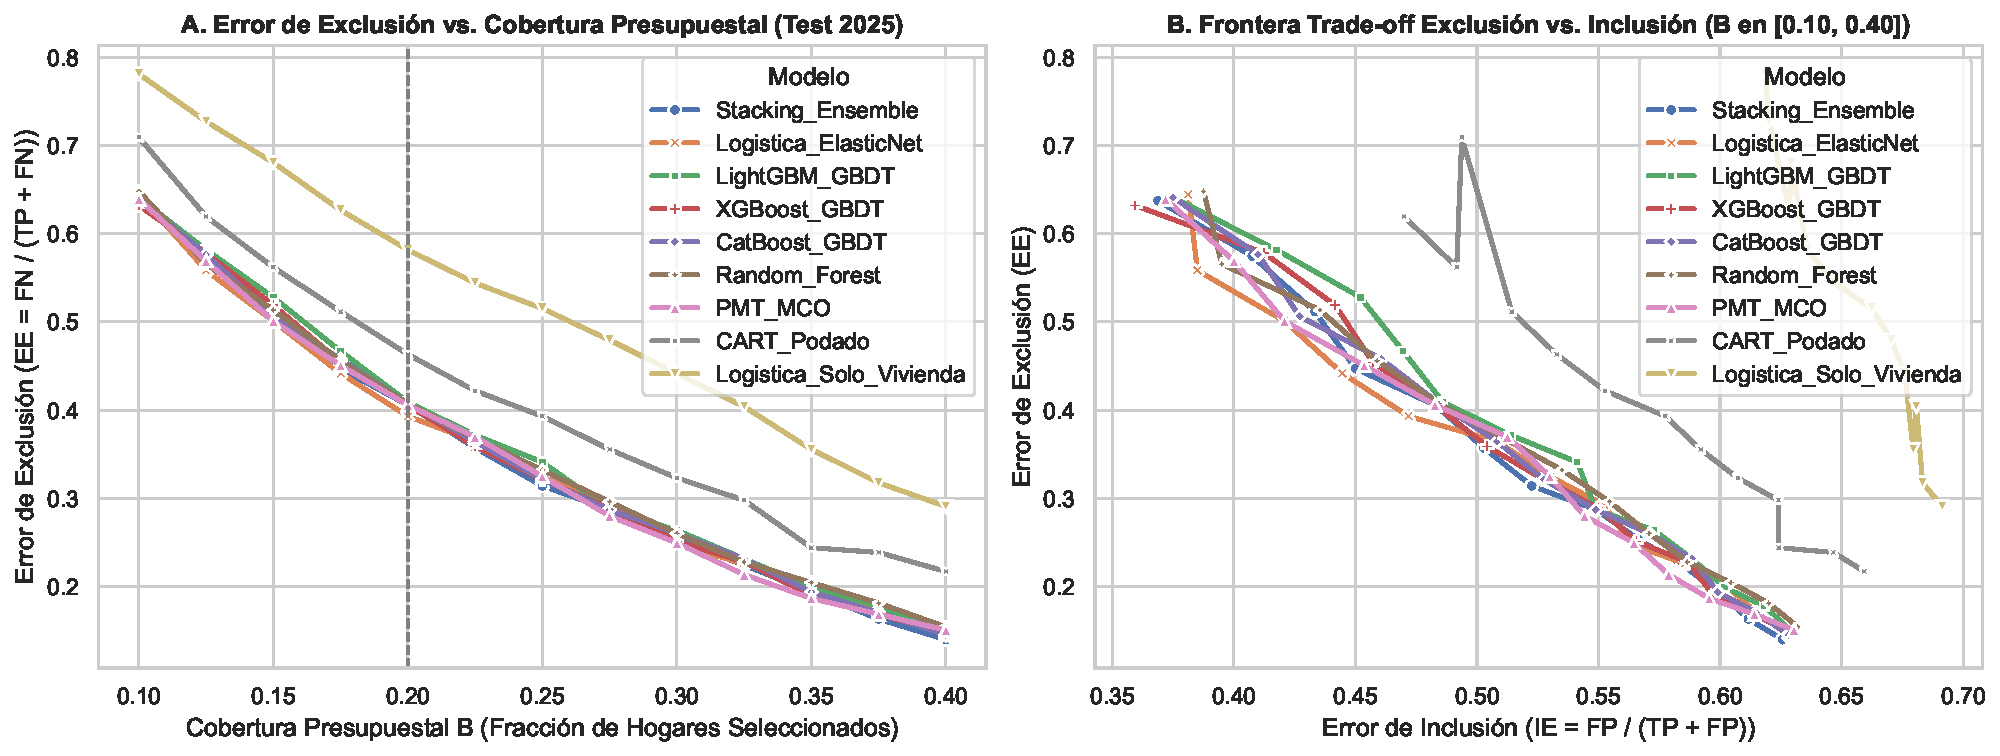
\includegraphics[width=0.90\textwidth,height=0.205\textheight,keepaspectratio]{figures/ee_ie_curves_2025.pdf}
\caption{Evaluación operativa fuera de tiempo en ENAHO 2025 ($N=3{,}199$). Panel A: Error de Exclusión ($\text{EE}$) en función de la cobertura presupuestal $B \in [0.10, 0.40]$. Panel B: Frontera de intercambio entre Error de Exclusión ($\text{EE}$) y Error de Inclusión ($\text{IE}$).}
\label{fig:ee_ie_2025}
\end{figure*}

La Figura~\ref{fig:ee_ie_2025} muestra que, a lo largo de todo el rango presupuestal $B \in [0.10, 0.40]$, las curvas de exclusión e inclusión de \texttt{Stacking\_Ensemble}, \texttt{Logistica\_ElasticNet}, \texttt{PMT\_MCO}, \texttt{XGBoost\_GBDT}, \texttt{CatBoost\_GBDT}, \texttt{LightGBM\_GBDT} y \texttt{Random\_Forest} se superponen casi por completo, reduciendo el error de exclusión desde $\sim 0.64$ en $B=0.10$ hasta $\sim 0.40$ en $B=0.20$ y $\sim 0.14$ en $B=0.40$. Por el contrario, un árbol individual podado (\texttt{CART\_Podado}, $\text{EE}_{B=20\%}=0.4632$) sufre una pérdida notable de eficiencia y las líneas base solo vivienda mantienen errores de exclusión superiores a $0.58$ en $B=0.20$.

\subsection{Contraste formal de hipótesis H1--H4 mediante Cluster Bootstrap}

La Tabla~\ref{tab:hipotesis_bootstrap} reporta el contraste de las cuatro hipótesis mediante \textit{cluster bootstrap} (1,000 réplicas remuestreadas a nivel de los 704 conglomerados de 2024 y 601 de 2025), aplicando con rigor la distinción entre corroboración al 95\% de confianza y cumplimiento en estimación puntual:

\begin{table}[htbp]
\centering
\caption{Contraste de hipótesis $H_1$--$H_4$ en ENAHO 2025 por \textit{cluster bootstrap} (1,000 réplicas).}
\label{tab:hipotesis_bootstrap}
\fontsize{6.1}{7.5}\selectfont
\setlength{\tabcolsep}{1.6pt}
\begin{tabular}{L{2.48cm}cccL{1.75cm}}
\toprule
\textbf{Hipótesis / Contraste} & \textbf{Obs.} & \textbf{IC95\% Inf.} & \textbf{IC95\% Sup.} & \textbf{Veredicto} \\
\midrule
\multicolumn{5}{l}{\textit{\textbf{H1: Ganancia de representación $\Delta\text{PR-AUC}_{2025} \ge +0.12$}}} \\
XGBoost $-$ RF\_Viv & $+0.2316$ & $+0.1891$ & $+0.2677$ & Corroborada (95\%) \\
CatBoost $-$ RF\_Viv & $+0.2236$ & $+0.1822$ & $+0.2630$ & Corroborada (95\%) \\
LightGBM $-$ RF\_Viv & $+0.2219$ & $+0.1794$ & $+0.2598$ & Corroborada (95\%) \\
Stacking $-$ Logit\_Viv & $+0.2201$ & $+0.1789$ & $+0.2605$ & Corroborada (95\%) \\
Logit\_EN $-$ Logit\_Viv & $+0.2102$ & $+0.1689$ & $+0.2514$ & Corroborada (95\%) \\
\midrule
\multicolumn{5}{l}{\textit{\textbf{H2: Equivalencia $|\Delta\text{EE}_{B=20\%}| \le 0.035$ (IC95\% en $\pm 0.035$)}}} \\
Stacking $-$ PMT\_MCO & $\phantom{+}0.0000$ & $-0.0227$ & $+0.0217$ & Corroborada (95\%) \\
Stacking $-$ Logit\_EN & $+0.0126$ & $-0.0126$ & $+0.0248$ & Corroborada (95\%) \\
XGBoost $-$ PMT\_MCO & $\phantom{+}0.0000$ & $-0.0246$ & $+0.0269$ & Corroborada (95\%) \\
XGBoost $-$ Logit\_EN & $+0.0126$ & $-0.0151$ & $+0.0321$ & Corroborada (95\%) \\
CatBoost $-$ Logit\_EN & $+0.0144$ & $-0.0153$ & $+0.0342$ & Corroborada (95\%) \\
RF $-$ PMT\_MCO & $+0.0018$ & $-0.0239$ & $+0.0326$ & Corroborada (95\%) \\
LightGBM $-$ PMT\_MCO & $+0.0036$ & $-0.0179$ & $+0.0375$ & Punto (IC $>0.035$) \\
LightGBM $-$ Logit\_EN & $+0.0162$ & $-0.0094$ & $+0.0415$ & Punto (IC $>0.035$) \\
\midrule
\multicolumn{5}{l}{\textit{\textbf{H3: Punto operativo 2025 ($\tau_{2024}$: $\text{Rec}\ge 0.70$, $\text{Prec}\ge 0.40$)}}} \\
Stacking Recall ($\tau=0.206$) & $\phantom{+}0.7110$ & $\phantom{+}0.6678$ & $\phantom{+}0.7515$ & Punto (IC $<0.70$) \\
Stacking Prec. ($\tau=0.206$) & $\phantom{+}0.4573$ & $\phantom{+}0.4217$ & $\phantom{+}0.4923$ & Corroborada (95\%) \\
LightGBM Recall ($\tau=0.395$) & $\phantom{+}0.7092$ & $\phantom{+}0.6696$ & $\phantom{+}0.7488$ & Punto (IC $<0.70$) \\
LightGBM Prec. ($\tau=0.395$) & $\phantom{+}0.4530$ & $\phantom{+}0.4166$ & $\phantom{+}0.4875$ & Corroborada (95\%) \\
Logit\_EN Recall ($\tau=0.374$) & $\phantom{+}0.7289$ & $\phantom{+}0.6856$ & $\phantom{+}0.7683$ & Punto (IC $<0.70$) \\
\midrule
\multicolumn{5}{l}{\textit{\textbf{H4: Estabilidad temporal $\Delta_{\text{temp}} = \text{PR}_{2024} - \text{PR}_{2025} \le 0.05$}}} \\
LightGBM\_GBDT & $+0.0022$ & $-0.0573$ & $+0.0618$ & Punto (IC $>0.05$) \\
XGBoost\_GBDT & $+0.0054$ & $-0.0508$ & $+0.0658$ & Punto (IC $>0.05$) \\
Stacking\_Ensemble & $+0.0080$ & $-0.0496$ & $+0.0708$ & Punto (IC $>0.05$) \\
PMT\_MCO (OLS/Ridge) & $+0.0162$ & $-0.0429$ & $+0.0773$ & Punto (IC $>0.05$) \\
Logistica\_ElasticNet & $+0.0253$ & $-0.0352$ & $+0.0872$ & Punto (IC $>0.05$) \\
\bottomrule
\end{tabular}
\end{table}

\begin{itemize}
    \item \textbf{H1 corroborada al 95\%:} los seis contrastes superan ampliamente el umbral de $+0.12$, con ganancias observadas de $+0.2102$ a $+0.2316$ y límites inferiores del $\text{IC}_{95\%}$ entre $+0.1689$ y $+0.1891$.
    \item \textbf{H2 corroborada al 95\% para \texttt{Stacking\_Ensemble}, \texttt{XGBoost\_GBDT} y \texttt{CatBoost\_GBDT} (y cumplida en punto para \texttt{LightGBM\_GBDT}):} el ganador \texttt{Stacking\_Ensemble} iguala exactamente el error de exclusión de \texttt{PMT\_MCO} ($\Delta\text{EE}=0.0000$, $\text{IC}_{95\%} [-0.0227, +0.0217]$) y difiere en $+0.0126$ de \texttt{Logistica\_ElasticNet} ($\text{IC}_{95\%} [-0.0126, +0.0248]$), manteniendo todo su intervalo dentro de $\pm 0.035$, al igual que \texttt{XGBoost\_GBDT} y \texttt{CatBoost\_GBDT}. En \texttt{LightGBM\_GBDT}, la diferencia puntual es mínima ($+0.0036$ frente a \texttt{PMT\_MCO} y $+0.0162$ frente a logística), pero el extremo superior del $\text{IC}_{95\%}$ ($+0.0375$ y $+0.0415$) rebasa el margen de $+0.035$.
    \item \textbf{H3 corroborada en estimación puntual en los 7 modelos principales (y al 95\% en precisión):} gracias a la imputación espacial jerárquica (\texttt{CONGLOME}$\rightarrow$\texttt{UBIGEO}$\rightarrow$global), que eliminó la asimetría entre CV 2024 y OOT 2025 en hogares secundarios, los siete modelos principales alcanzan simultáneamente $\text{Recall}_{2025} \ge 0.70$ (entre $0.7002$ y $0.7289$) y $\text{Precisión}_{2025} \ge 0.40$ (entre $0.4457$ y $0.4619$) con su umbral $\tau_{2024}$ congelado; la precisión supera $0.40$ incluso en el extremo inferior del $\text{IC}_{95\%}$ ($\ge 0.411$), mientras que el límite inferior del recall se sitúa entre $0.658$ y $0.686$.
    \item \textbf{H4 cumplida en estimación puntual, pero no demostrada al 95\%:} la degradación interanual observada es muy reducida ($+0.0022$ en \texttt{LightGBM\_GBDT}, $+0.0054$ en \texttt{XGBoost\_GBDT}, $+0.0080$ en \texttt{Stacking\_Ensemble} y $+0.0253$ en \texttt{Logistica\_ElasticNet}, todas $\le 0.05$), pero la varianza de muestreo entre conglomerados independientes hace que el límite superior del $\text{IC}_{95\%}$ alcance entre $+0.0618$ y $+0.0872$.
\end{itemize}

\subsection{Explicabilidad global con TreeSHAP y consolidación para inferencia}

\begin{figure}[htbp]
\centering
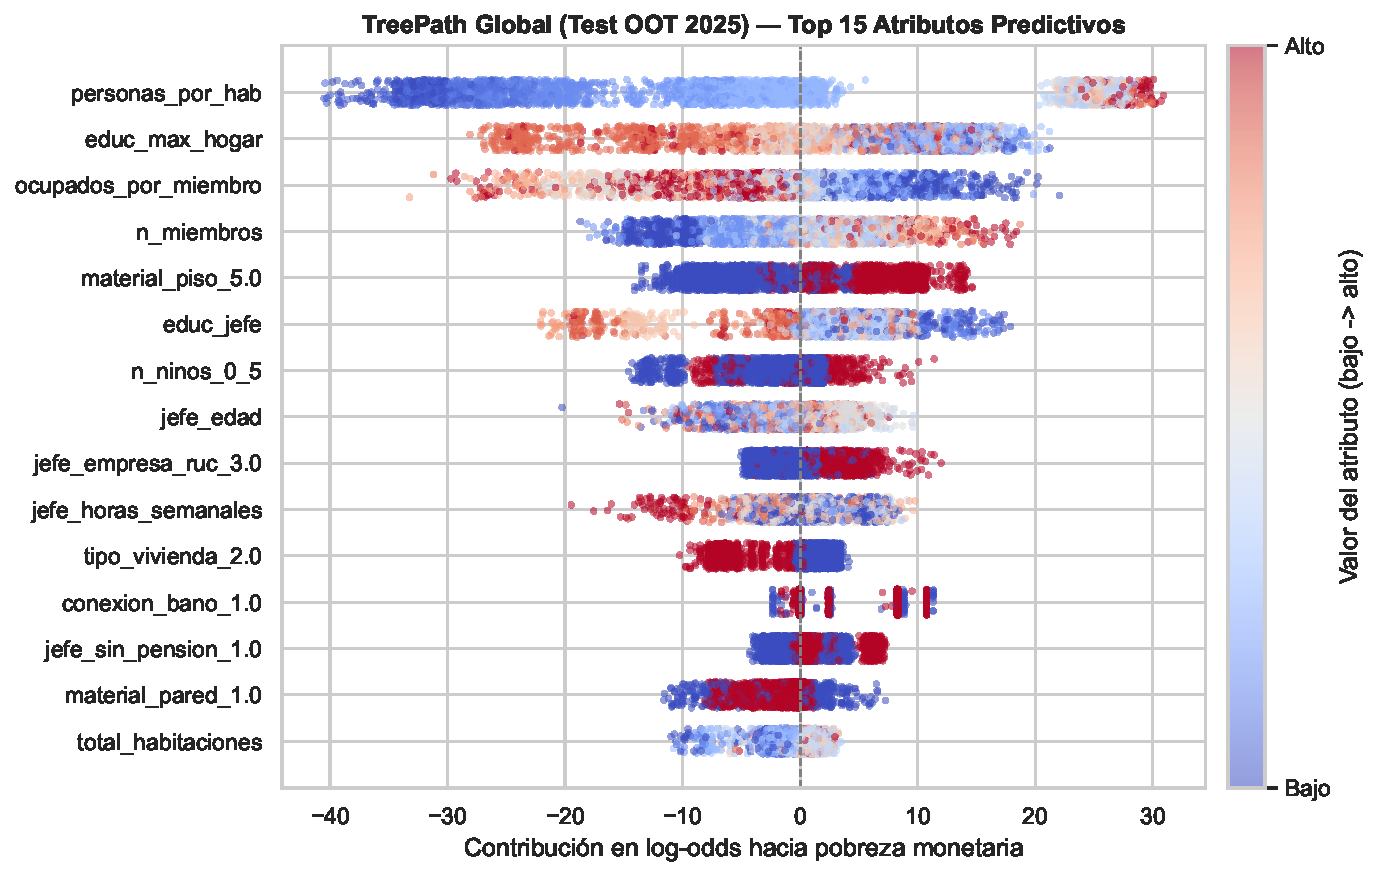
\includegraphics[width=0.92\columnwidth]{figures/shap_beeswarm_2025.pdf}
\caption{Explicabilidad global TreeSHAP en espacio log-odds sobre ENAHO 2025 ($N=3{,}199$, Top 15 atributos codificados).}
\label{fig:shap_beeswarm}
\end{figure}

La descomposición exacta mediante TreeSHAP \cite{lundberg2020local} sobre \texttt{LightGBM\_GBDT} en el conjunto de prueba 2025 (Figura~\ref{fig:shap_beeswarm}, con contribuciones individuales bien escaladas en $[-2.19, +1.81]$ log-odds) revela que los tres bloques no habitacionales concentran el \textbf{54.31\%} de la importancia predictiva total ($\sum |\phi| = 3.7986$): \textbf{Empleo y Formalidad ($\text{M05}/\Phi$)} aporta el \textbf{22.35\%} ($0.8488$), \textbf{Demografía ($\text{M02}$)} el \textbf{16.72\%} ($0.6350$) y \textbf{Educación ($\text{M03}$)} el \textbf{15.24\%} ($0.5791$). El bloque de \textbf{Vivienda y Hacinamiento ($\text{M01}/\Phi$)} representa el \textbf{45.69\%} restante ($1.7357$), compuesto por un \textbf{26.50\%} de infraestructura física pura de la vivienda y un \textbf{19.19\%} proveniente del ratio de hacinamiento (\texttt{personas\_por\_hab}, primera variable individual con $|\phi|=0.7290$), seguida por \texttt{material\_piso} ($10.30\%$), \texttt{ocupados\_por\_miembro} ($8.88\%$), \texttt{educ\_max\_hogar} ($8.76\%$), \texttt{n\_miembros} ($8.59\%$), \texttt{educ\_jefe} ($6.48\%$), \texttt{jefe\_empresa\_ruc} ($4.48\%$) y \texttt{jefe\_sin\_pension} ($4.13\%$).

\begin{figure*}[!t]
\centering
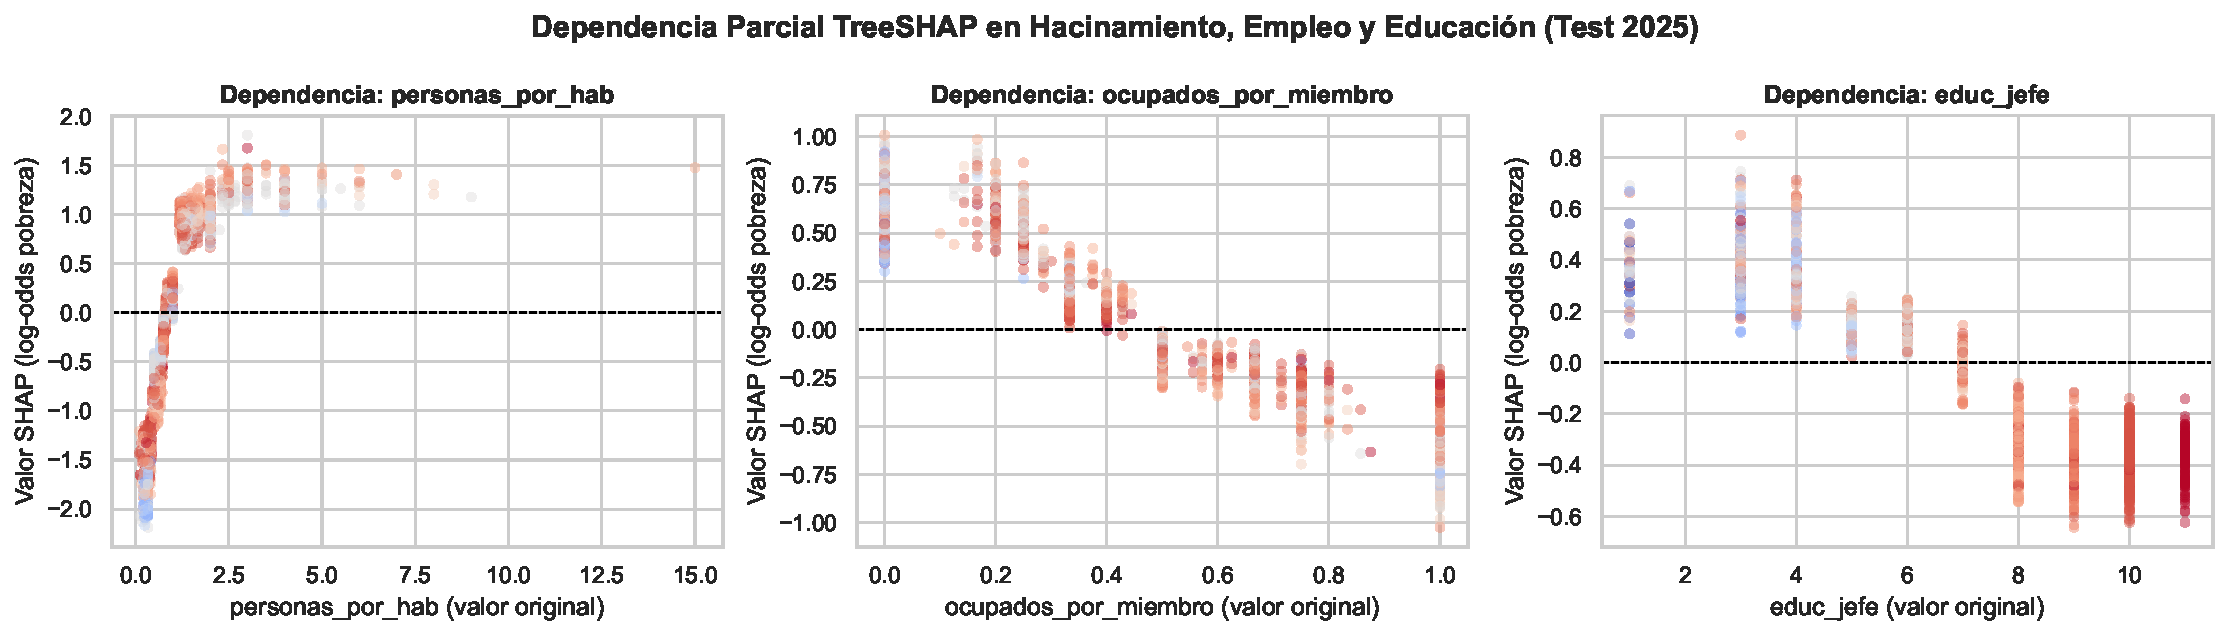
\includegraphics[width=0.90\textwidth,height=0.185\textheight,keepaspectratio]{figures/shap_dependence_2025.pdf}
\caption{Gráficos de dependencia parcial TreeSHAP en ENAHO 2025 para las tres dimensiones estructurales principales: hacinamiento (\texttt{personas\_por\_hab}), inserción laboral (\texttt{ocupados\_por\_miembro}) y nivel educativo del jefe (\texttt{educ\_jefe}), coloreados por el máximo nivel educativo del hogar.}
\label{fig:shap_dependence}
\end{figure*}

Los gráficos de dependencia parcial (Figura~\ref{fig:shap_dependence}) evidencian relaciones no lineales con sentido económico directo: (i) en \texttt{personas\_por\_hab}, vivir con menos de $1.0$ persona por habitación reduce el riesgo hasta $-2.1$ log-odds, pero superar el umbral crítico de $1.5$ a $2.5$ personas por habitación dispara la contribución positiva hasta $+1.5$ log-odds con saturación posterior; (ii) en \texttt{ocupados\_por\_miembro}, la contribución cae monotónicamente desde $+0.75$ log-odds en hogares sin perceptores hasta $-0.70$ cuando más de la mitad del hogar trabaja; y (iii) en \texttt{educ\_jefe}, alcanzar educación superior técnica o universitaria (códigos $\ge 8$) invierte el signo hacia valores protectores de $-0.35$ a $-0.55$ log-odds. Finalmente, para la puesta en producción se consolidaron los $N=7{,}289$ hogares físicos únicos de 2024--2025 en un artefacto regularizado (\texttt{models/winner\_bundle.joblib}) cuya auditoría Out-Of-Fold confirma ausencia de sobreajuste ($\text{PR-AUC Train}=0.6211$, $\text{OOF}=0.5729$, $\text{Gap}=0.0482 < 0.05$, $\text{ROC-AUC OOF}=0.8620$), clasificando correctamente perfiles de prueba desde hogares vulnerables hacinados ($91.44\%$ de probabilidad, percentil $100$) y hogares secundarios en Chorrillos evaluados vía mediana distrital ($59.52\%$, percentil $92.1$) hasta hogares formales estables ($4.17\%$, percentil $4.8$).
